\section{Common Image Operations}
In this study, we wish to see how the primitive operations of addition and multiplication supported by homomorphic cryptosystems can be applied to image processing operations. These operations are performed on digital images. We can represent a digital image $R$ as an $M \times N$ matrix of pixel intensity values, each value in the range $\left[0, L-1\right]$, for some positive integer $L$. There are two types of basic operations in image processing, intensity transformations, which map an intensity value to another, spatial filters which assist in operations such as edge detection and image blurring.

\subsection{Intensity Transformation}
To define an intensity transformation on an image $R$, we define a function $T$ which maps a pixel value $r$ to a new value $r^\prime$, which we can write as $r^\prime = T\left(r\right)$. This function is then applied to every pixel in $R$. Examples of intensity transformations are image negation, log transformation, and power-law transformation.

Image negation is an example of an intensity transformation, where the resulting image would be similar to a photographic negative~\cite{gonzalez_digital_2008}. An image negation operation is defined as:
\begin{equation}
    T\left(r\right) = L-1-r
\end{equation}

The log transformation is used to enhance dark pixels or increase the dark details of an image by mapping low intensity values to a wider range of values~\cite{gonzalez_digital_2008}. This has the general form
\begin{equation}
    T\left(r\right) = c \log\left(1 + r\right)
\end{equation}
where $c$ is a constant and $r \ge 0$.

The power-law transformation is a family of transformations that have the form
\begin{equation}
    T\left(r\right) = c r^{\gamma}
\end{equation}
where $c>0$ and $\gamma > 0$. This is especially useful since many image capture and output devices such as cameras, printers and displays follow a similar power law to relate physical perceived light intensity and digital pixel intensity values. A power-law transformation defined by the above equation can calibrate the operation on these devices in a process called \textit{gamma correction}. This ensures reproducibility and accuracy of images being displayed~\cite{gonzalez_digital_2008}.

In the \textit{CryptoImg} software library, of the intensity transformations above, only image negation was implemented under a homomorphic cryptosystem~\cite{ziad_cryptoimg:_2016}. To implement these intensity transformations using addition and multiplication in a homomorphic system, it is necessary to approximate the logarithm and exponential functions, which may result in higher computational overhead. In our software library implementation, we aim to investigate the overhead required to approximate these functions.

\subsection{Spatial Filtering}
Many common image operations are expressed as \textit{spatial filters}. Spatial filters are operators which determine output pixels using information from neighboring input pixels. To apply a spatial filter to obtain a resulting image $R^\prime$, a convolution is performed between an $m \times n$ matrix $k$, called a kernel, and the original $M\times N$ image $R$.
A convolution between a kernel $k$ and image $R$ which yields a resulting image $R^\prime$, denoted as $R^\prime = k \ast R$, is defined by
\begin{align} \label{eq:spatialfilter}
	R^\prime(x,y) = \sum_{s=1}^m{\sum_{t=1}^n{k(s,t)R(x+s,y+t)}}, \text{ for all } 0\leq x \leq M, 0 \leq y \leq N,
\end{align}
where $A(x,y)$ represents the entry at the $x$th row and $y$th column of a matrix $A$.

\begin{figure*}[!ht]
    \centering
    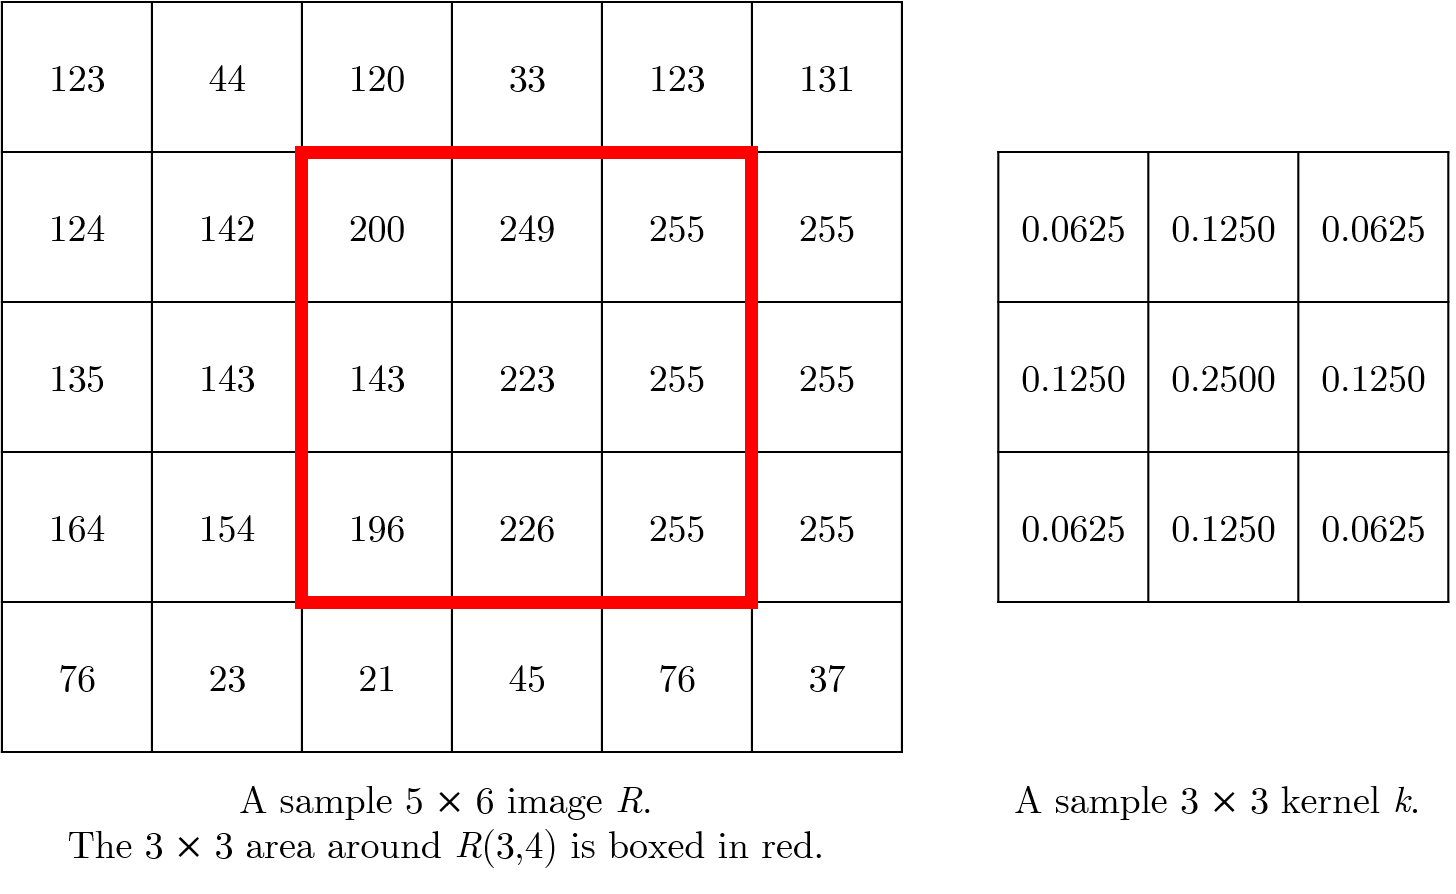
\includegraphics[width=\textwidth,\keepaspectratio]{Figures/SpatialFilter.png}
    \caption{(a) A sample image $R$. (b) A sample kernel $k$.}
    \label{fig:spatialfilter}
\end{figure*}
For example, using the image and kernel given in Figure \ref{fig:spatialfilter}, we can calculate the value in the third row and fourth column of the resulting image $R^\prime$ as follows:
\begin{align*}
	R^\prime(3,4) &= \sum_{s=1}^m{\sum_{t=1}^n{k(s,t)R(3+s,4+t)}}\\
	&= (0.0625\times 200) + (0.1250\times 249) + (0.0625\times 255) \\
	&+ (0.1250\times 143) + (0.2500\times 223) + (0.1250\times 255) \\
	&+ (0.0625\times 196) + (0.1250\times 236) + (0.0625\times 255)\\
	&= 223.
\end{align*}
Since spatial filters take values from a contiguous region of pixels, this presents a difficulty in homomorphic cryptosytems: in order for spatial filters to be performed, the location of each pixel relative to neighboring pixels has to be preserved. This was performed in the implementation of spatial filters in the \textit{CryptoImg} library~\cite{ziad_cryptoimg:_2016}. We wish to implement spatial filters using a similar approach, and assess how preserving spatial correlation between pixels can impact the security of the encrypted image.

\subsection{Common Spatial Filtering Kernels}
Edge detection is used to find and determine the boundaries in an image, commonly used in applications such as image segmentation and feature extraction. This works by detecting so-called \textit{edges}, areas that have abrupt changes in intensity.
One common method of performing edge detection is the Sobel operator, which uses two spatial filters to approximate the gradient in an image. Given an image $R$, and the kernels
\begin{equation}
    g_x =
    \begin{bmatrix}
        -1 & 0 & 1 \\
        -2 & 0 & 2 \\
        -1 & 0 & 1
    \end{bmatrix}
    \qquad\text{and}\qquad
    g_y =
    \begin{bmatrix}
        1 & 2 & 1 \\
        0 & 0 & 0 \\
        -1 & -2 & -1
    \end{bmatrix},
\end{equation}
$g_x \ast R$ yields the horizontal component of the gradient, while $g_y \ast R$ yields the vertical component of the gradient.

There are also spatial filters that perform image smoothing (such as Gaussian blur and box blur, which use the kernels $b_g$ and $b$ respectively in Equation~\ref{eqn:smooth-filters}) and image sharpening~\cite{gonzalez_digital_2008}.
\begin{equation}
    \label{eqn:smooth-filters}
    b_g = \frac{1}{16}
    \begin{bmatrix}
        1 & 2 & 1 \\
        2 & 4 & 2 \\
        1 & 2 & 1
    \end{bmatrix}
    \qquad
    b = \frac{1}{9}
    \begin{bmatrix}
        1 & 1 & 1 \\
        1 & 1 & 1 \\
        1 & 1 & 1
    \end{bmatrix}
\end{equation}
% Should I put a table of other kernels too?
